\textbf{\emph{David L.}}

\emph{Simulation should be distributed across multiple Compute facilities. The raw data reconstruction should likewise include multiple sites. In the model where we do calibrations and reconstruction in ``real time'' the data will need to be streamed to multiple sites if we are to federate the processing of raw data. This should discuss federating those resources.}

\emph{See slide 4 of Nhan Tran's talk at AI4EIC.}

\emph{The final raw data (as defined by DOE rules) must have multiple copies. Could this be done by storing one at BNL wile simultaneously transferring a copy to JLab for storage? Other sites?}

\emph{Need estimates on total bandwidth needed from BNL, number of remote sites, and bandwidth/storage needed from each.}

%-------------------------------------------------------------------
\subsection{Raw Data Compute}
Processing of EIC data will occur over multiple sites which will include HTC facilities at both BNL and JLab and possibly others. The plan calls for processing the raw data into reconstructed objects such as tracks, jets, and calorimeter clusters within 2-3 weeks of acquisition. The bulk of the few week latency will be due to the time it takes to calibrate the data so that reconstruction may occur. Figure \ref{fig:federated_offsite_example} illustrates how such a scheme could work. The raw data read from the Streaming DAQ system will need to be reduced over multiple filtering and compression stages to a rate that is reasonable to transport offsite from BNL using its external network connection. Table \ref{tab:reduction_factors} lists the stages and with ingoing and outgoing rates and their respective reduction factors. Potential technologies that could be applied at each stage are also listed.

The DOE lab systems are connected via the ESNet unclassified network for scientific research\cite{ESNet}. As of 2021, BNL has a 400Gbps connection to ESNet and JLab has dual 10Gbps connections. In 2022 or 2023, JLab is anticipated to increase its bandwidth to at least 100Gbps. When the EIC begins collecting data around 2030, one may expect a 1Tbps bandwidth between the two labs. This is an order of magnitude higher than the anticipated raw data rate from the ECCE. Thus, transfer of the entire raw data set offsite from BNL in 2030 seems reasonable.


\begin{figure}[hbt!]
 \begin{center}
   \raisebox{0.5mm}{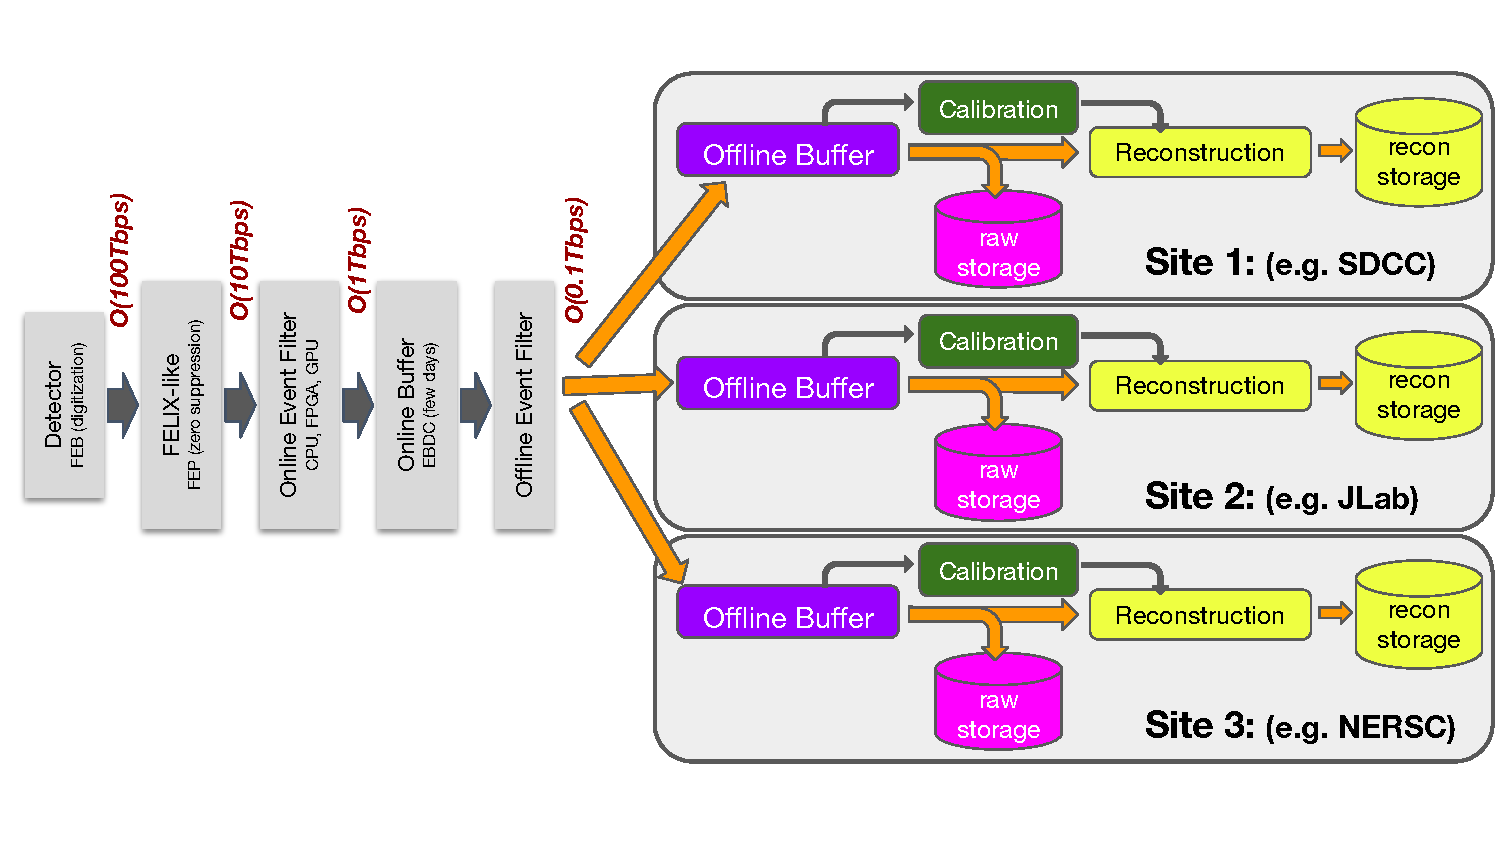
\includegraphics[clip, width=0.99\linewidth]{figs/figure_federated_offsite_example.pdf}}
  \caption[Example of federated processing of data in near real-time using multiple sites.]{\label{fig:federated_offsite_example} Data flow from detector to reconstructed object files (left to right). This diagram illustrates how raw data may be distributed to multiple sites in near-real time. On the left side of the plot, multiple filter and buffering stages are used to reduce the data rate. On the right, the data is distributed to multiple facilities.
  Each facility would store a portion of the raw data. It would also need to keep the data live (e.g. on disk) long enough for it to be calibrated and then processed by the reconstruction software.}
 \end{center}
\end{figure}

\begin{table}[htb!]
    \centering
    \begin{tabular}{p{4cm}|c|c|c}
        \hline
        Stage                        & Input/Output    & Reduction Factor & Technology options \\
        \hline
        \hline
        Compute Interface (e.g. FELIX) & 100Tbps/10Tbps  & $\times 10^{-1}$ & FPGA \\
        \hline
        Online Event Filter          & 10Tbps/1Tbps    & $\times 10^{-1}$ & FPGA, (GPU), CPU\\
        \hline
        Online Buffer                & 1Tbps/0.5Tbps   & $\times 2x10^{-1}$  & $<disk>$ \\
        \hline
        Offline Event Filter         & 0.5Tbps/100Gbps & $\times 5x10^{-1}$  & FPGA, GPU, CPU \\
        \hline
        Reconstruction               & 100Gbps/10Gbps  & $\times 10^{-1}$ & (FPGA), GPU,CPU\\
        \hline
        \hline
        \textbf{Total}               & \textbf{100Tbps/10Gbps} & \textbf{$\times 10^{-4}$} & \\
        \hline
    \end{tabular}
    \caption{Data rates and reduction factors for proposed near real time data flow. Estimated data rate from ECCE detector is $\mathcal{O}(100Tbps)$. Raw storage will be $\mathcal{O}(100Gbps)$. Reconstructed object storage will be $\mathcal{O}(10Gbps)$. Parentheses indicate technologies that could be used, but seem less likely choices.}
    \label{tab:reduction_factors}
\end{table}

%-------------------------------------------------------------------
\subsection{Simulation Compute}

